% ID: SEL-D0012-BA-E01
% ESTADO: validada. S013; tres pasadas del mismo autor, sin segundo revisor.
\textbf{Modelo y frontera estricta.}\par\nopagebreak[4]
Sean $x$ misiones e $y$ programas. Midiendo el presupuesto en unidades de $100000$ euros, las condiciones son
\[
\boxed{20<2x+y\leq24,\qquad x\geq4,\qquad y\geq2x.}
\]
La no negatividad ya queda implicada. Se maximiza $F=0.6x+0.4y$. En el contexto se requieren cantidades enteras; entonces superar $20$ equivale a $2x+y\geq21$. Primero representamos el modelo continuo conservando la desigualdad estricta original.

\textbf{Recinto y vértices de su cierre.}\par\nopagebreak[4]
Las cuatro intersecciones que delimitan el cierre son
\[
(4,12),\quad(5,10),\quad(6,12),\quad(4,16).
\]
Los dos primeros puntos y todo el lado que los une cumplen $2x+y=20$ y \textbf{están excluidos}. Los otros lados pertenecen al recinto, salvo esos extremos excluidos. La figura usa línea discontinua y círculos abiertos para esa frontera.
\begin{center}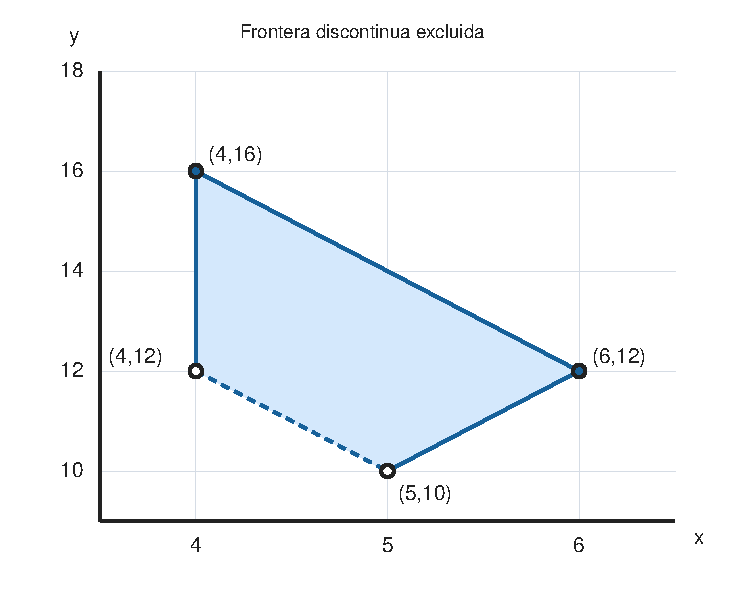
\includegraphics[width=0.57\linewidth]{recursos/figuras/s013-region.pdf}\end{center}

\textbf{Máximo y comprobación global.}\par\nopagebreak[4]
No aplicamos sin más un teorema para polígonos cerrados al recinto abierto. Para cualquier punto factible,
\[
F=0.4(2x+y)-0.2x\leq0.4\cdot24-0.2\cdot4=8.8.
\]
La igualdad exige $2x+y=24$ y $x=4$, de donde $y=16$. Es un punto factible: inversión $2.4$ millones, superior a $2$ millones; $4\leq16/2$. Además, ambas cantidades son enteras.
\[
\boxed{4\text{ misiones y }16\text{ programas};\qquad F_{\max}=8.8.}
\]
El máximo es único. En los cuatro vértices del cierre, los valores son $7.2$, $7$, $8.4$ y $8.8$, respectivamente. Los dos primeros puntos no son factibles. $F$ es la valoración dada, sin unidades monetarias.
